% !TEX program = xelatex
%% Requires compilation with XeLaTeX or LuaLaTeX
\documentclass[10pt,xcolor={table,dvipsnames},t]{beamer}
\usepackage{biblatex}
\usepackage{caption}
\setbeamertemplate{caption}[numbered]
\addbibresource{reference.bib}
\usepackage{hyperref}
\hypersetup{ 
pdfpagemode=FullScreen,  
colorlinks=true,linkcolor=blue}
\usepackage{enumerate}

\usepackage{listings}
\usepackage{xcolor}

\definecolor{codegreen}{rgb}{0,0.6,0}
\definecolor{codegray}{rgb}{0.5,0.5,0.5}
\definecolor{codepurple}{rgb}{0.58,0,0.82}
\definecolor{backcolour}{rgb}{0.95,0.95,0.92}

\lstdefinestyle{mystyle}{
    backgroundcolor=\color{backcolour},   
    commentstyle=\color{codegreen},
    keywordstyle=\color{magenta},
    numberstyle=\tiny\color{codegray},
    stringstyle=\color{codepurple},
    basicstyle=\ttfamily\footnotesize,
    breakatwhitespace=false,         
    breaklines=true,                 
    captionpos=b,                    
    keepspaces=true,                 
    numbers=left,                    
    numbersep=5pt,                  
    showspaces=false,                
    showstringspaces=false,
    showtabs=false,                  
    tabsize=2
}

\lstset{style=mystyle}

\usetheme{UCBerkeley}

\title[Your Short Title]{STMC HKOI Training}
\subtitle{Lesson 1: Hello World}
\author{Chan Yan Mong}
%\institute{}
\date{\today}

\begin{document}

\begin{frame}
  \titlepage
\end{frame}

% Uncomment these lines for an automatically generated outline.
%\begin{frame}{Outline}
%  \tableofcontents
%\end{frame}

\section{Class Goal}

\begin{frame}{Goal today}

\begin{itemize}
  \item Install python
  \item Run your first program \texttt{helloworld.py}
  \item Understand different parts of \texttt{helloworld.py}
  \item Use VSCode as an integrated development environment (IDE) for coding
\end{itemize}
%\begin{block}{Examples}
%Some examples of commonly used commands and features are included, to help you get started.
%\end{block}

\end{frame}

\section{Installing python}

\begin{frame}{Installing python}
  \begin{itemize}
    \item As mentioned before, a interpreter is need to run our code
    \item Now we shall learn how to install interpreter for python
  \end{itemize}
\end{frame}


\begin{frame}{Installing python}
  \begin{columns}
    \column{0.8\textwidth}
    \begin{enumerate}[Step 1:]
      \item Go to Python's website (\href{https://www.python.org/}{https://www.python.org/})
      \item Click \texttt{Downloads} and choose \texttt{Python 3.X}
      \item Follow the link and download the installer
    \end{enumerate}
  \end{columns}
  
\end{frame}

\begin{frame}{Installing python}
  \begin{columns}
    \column{0.8\textwidth}
    \begin{enumerate}[Step 1:]
      \setcounter{enumi}{3}
      \item Double-click the installer and follow the installation instructions. Wait until it says installation success
      \item Close the installer window
    \end{enumerate}
  \end{columns}
\end{frame}

\begin{frame}{Installing python}
  \begin{columns}
    \column{0.8\textwidth}
    \begin{enumerate}[Step 1:]
      \setcounter{enumi}{5}
      \item Double click the installer again. Tick "Add Python 3.9 to PATH" and click "Custom Installation"
    \end{enumerate}
  \end{columns}
  \vspace{1mm}
  \begin{figure}
    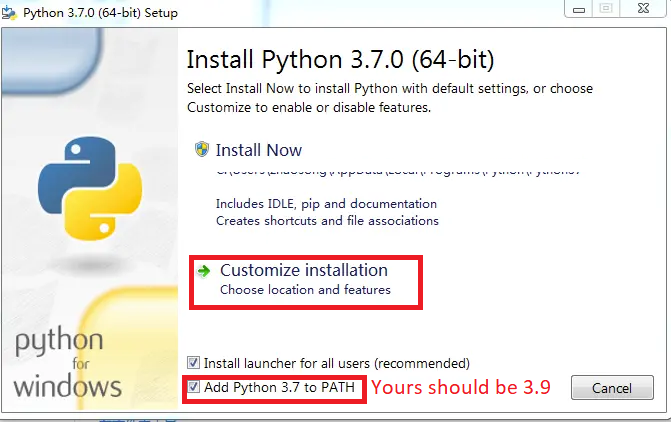
\includegraphics[width=0.7\textwidth]{img/install-menu.png}
  \end{figure}
\end{frame}

\begin{frame}{Installing python}
  \begin{columns}
    \column{0.8\textwidth}
    \begin{enumerate}[Step 1:]
      \setcounter{enumi}{6}
      \item Tick the following and press "Next" to install
    \end{enumerate}
  \end{columns}
  \vspace{1mm}
  \begin{figure}
    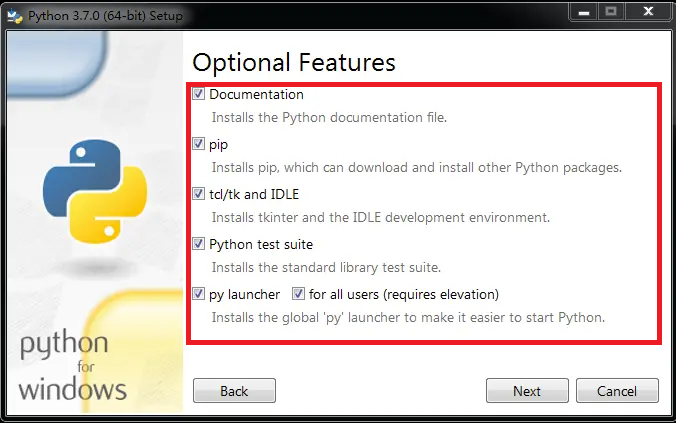
\includegraphics[width=0.7\textwidth]{img/optional-feature.png}
  \end{figure}
\end{frame}

\section{Running your first program}
\begin{frame}{Running your first program (I)}
  \begin{columns}
    \column{0.8\textwidth}
    \begin{enumerate}[Step 1:]
      \item Download \texttt{helloworld.py} from course webpage and paste it on your Desktop
      \item Open CMD (Windows) / Terminal (Mac) 
      \item Type \texttt{cd Desktop} (Windows) or \texttt{cd \char`~/Desktop/} (Mac)
      \item Type \texttt{dir .} (Windows) or \texttt{ls .} (Mac). That should list all your files on Desktop, including \texttt{helloworld.py}
    \end{enumerate}
  \end{columns}
\end{frame}

\begin{frame}[fragile]{Running your first program (II)}
  Now run the following command:

  \begin{lstlisting}[language=Bash]
python helloworld.py
\end{lstlisting}
\vspace{1mm}
You should see the following results:
  \begin{lstlisting}
  Hello world!\end{lstlisting}
\end{frame}
\section{Understanding helloworld.py}
\begin{frame}[fragile]{Understand helloworld.py}
  Congrats, you just compile your first program. Now, let's open \texttt{helloworld.py} and see what's under the hood:
  \begin{lstlisting}[language=python]
print("Hello world!") # Printing Hello world
\end{lstlisting}
\end{frame}

\begin{frame}[fragile]{Experiments}
  Let's explore the function of different parts of the program by doing some experiments:
  \begin{itemize}
    \item Change "Hello World" to "Bye bye world" and rerun, what do you observe?
    \item Similar to the first line, add more \texttt{print} to see if you can print multiple lines
    \item Enter "Hello\textbackslash n World" and rerun, what do you observe? How about adding more "\textbackslash n"? What is the function of "\textbackslash n"?
    \item Change the text behind \# and recompile, does it change anything about the code? Now try to add \# before \texttt{print}, what happens?
  \end{itemize}
\end{frame}

\begin{frame}[fragile]{Explaining helloworld.py: print}
  \begin{itemize}
    \item \texttt{print} is a function used for printing things
    \item In \texttt{helloworld.py}, \texttt{print} is used to print our hello message "Hello world"
    \item You can also do something like this:
\begin{lstlisting}[language=python]
  print("Text 1", "Text 2", "Text 3")
\end{lstlisting}
    These text will be separated by spaces (Try it!)
    \item You can read more about \texttt{print} from the \href{https://docs.python.org/3/library/functions.html#print}{documentation}
  \end{itemize}
\end{frame}

\begin{frame}{Explaining helloworld.py: \textbackslash n}
  \begin{itemize}
    \item From your experiments, you can see that \textbackslash n is not printed literally as "\textbackslash" and  "n"
    \item \textbackslash n turns out are one of those we called \textbf{escape characters}
    \item Escape characters are \textit{treated differently} by computer 
    \item For example, \textbackslash n is interpreted as new line (Enter) by Python
    \item Usually it takes the form "\textbackslash"+"<another character>"
  \end{itemize}
\end{frame}

\begin{frame}{Explaining helloworld.py: \textbackslash n}
  Here are more escape characters. Try them out!
  \begin{table}[]
    \begin{tabular}{ll}
    \textbackslash{}n                & New Line         \\
    \textbackslash{}r                & Carriage Return  \\
    \textbackslash{}t                & Tab (Horizontal) \\
    \textbackslash{}\textbackslash{} & Backslash        \\
    \textbackslash{}'                & Single Quote     \\
    \textbackslash{}"                & Double Quote    
    \end{tabular}
    \end{table}
\end{frame}

\begin{frame}{Explaining helloworld.py : Comments}
  \begin{itemize}
    \item Those lines after \texttt{\#} are called \textbf{comments}
    \item They are ignored by compiler and will not affect how the code run
    \item Their are notes left by programmers to help himself/herself/others to understand the code 
    \item \textbf{For more complicated program, comments are necessary}. Otherwise, code will be very difficult to comprehend and debug
  \end{itemize}
\end{frame}

\begin{frame}[fragile]{Explaining helloworld.py : Comments}
  Another type of comments available in Python (and many other languages) is the \textbf{block comment}. They look something like this:
\begin{lstlisting}[language=python]
  # This is the single line comment we just saw

  """ 
     This is a block comment,
     anything inside this block will be ignored
  """

  """ This is also a block comment """
\end{lstlisting}
\end{frame}

\section{Using an IDE}
\begin{frame}{Using an IDE}
  \begin{itemize}
    \item As you can probably experience just now, using command line is sometimes a bit troublesome
    \item Hence programmers invented \textbf{integrated development environment (IDE)} to aid coding
    \item Here we will setup one of the most popular IDE / text editor on the market: \textbf{VSCode}
  \end{itemize}
\end{frame}

\begin{frame}{Setting up VSCode for Python}
  \begin{columns}
    \column{0.8\textwidth}
    \begin{enumerate}[Step 1:]
      \item Download \textbf{Visual Studio Code} from \href{https://code.visualstudio.com/}{https://code.visualstudio.com/}
      \item Follow the instructions in \href{https://code.visualstudio.com/docs/python/python-tutorial}{https://code.visualstudio.com/docs/python/python-tutorial} to install learn how to integrate python with VSCode
    \end{enumerate}
  \end{columns}
  
\end{frame}
\end{document}
